\section{Lecture 6}
\subsection{Clarification on BIBO Stability}
\begin{itemize}
	\item When we say a "bounded" signal, we mean that the amplitude of the signal is bounded at all times:
		\[
		|x(t)| < \infty \ \forall t \in \R
		\] 
		The same definition follows for discrete-time signals. 
	\item For LTI systems, we call the system BIBO stable if and only if its impulse \( h(t) \) is absolutely 
		integrable:
		\[
		\int_{-\infty}^{\infty} |h(t)| \diff t < \infty
		\] 
\end{itemize}
\subsection{Cross-Correlation}
\begin{itemize}
	\item The cross correlation between two signals \( r_{xy}(t) = r_{yx}(-t) \). To show this explicitly, we 
		look at the cross-correlation equation:
		\begin{align*}
			r_{xy}(t) &= \int_{-\infty}^{\infty} x(\tau)y(t + \tau) \diff \tau \\
			r_{yx}(t) &= \int_{-\infty}^{\infty} y(\tau) x(t + \tau) \diff \tau  
	\end{align*} 
	But for the second equation, we can define a \( \tau' = t + \tau\), so then we get: 
	\[
	r_{yx}(t) = \int_{-\infty}^{\infty} y(\tau' - t)x(\tau') \diff \tau' = \int_{-\infty}^{\infty} 
	x(\tau') y(-t + \tau') \diff \tau'
	\] 
	This looks like the first equation except we have \( -t \) instead of \( t \). Therefore, we have 
	\( r_{xy}(t) = r_{yx}(-t) \). The same works for discrete time: \( r_{xy}[n] = r_{yx}[-n] \). 
\end{itemize}

\subsection{More Convolution Properties} 
\begin{itemize}
	\item \textbf{Differentiation property:} Given \( y(t) = x(t) * h(t) \), then:
		\[
			\dv{t} y(t) = x(t) * \dv{h(t)}{t} = \dv{x(t)}{t} * h(t)
		\] 
	\item \textbf{Intergration Property:} Given \( y(t) = x(t) * h(t) \), we have:
		\[
		\int_{-\infty}^{t'} y(t) \diff  t = x(t) * \int_{-\infty}^{t'} h(\tau)\diff \tau 
		\] 
\end{itemize}
\subsection{Fourier Transform} 
\begin{itemize}
	\item The fourier transform came from the study of the heat equation, written as:
		\[
			c \rho \pdv{t} u(x, y, z, t) = k \left( \pdv[2]{x} + \pdv[2]{y} + \pdv[2]{z} \right) 
			u(x, y, z, t)
		\] 
		Fourier then claimed that the solution can be expanded in a series of sines with multiples of the variable. 
		In other word,s the solution is of the form:
		\[
		f(x) = \frac{1}{2a_0} + (a_1 \sin(x) + b_2 \cos(x)) + (a_2\sin(2x) + b_2\cos(2x)) + \cdots 
		\] 
	\item Recall the frequency response of an LTI system:
		\begin{center}
			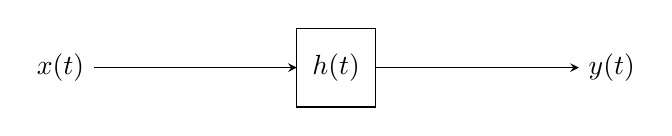
\begin{tikzpicture}
				\node (A) at (-3, 0) {\( x(t) \) };
				\node (B) at (4, 0) {\( y(t) \) };
				\draw[-stealth] (A) -- (0, 0);
				\draw (0, -0.5) rectangle node {\( h(t) \) } (1, 0.5);
				\draw[-stealth] (1, 0) -- (B);
			\end{tikzpicture}
		\end{center}
		Recall that we can characterize \( y(t) \) via a convolution: 
		\[
		y(t) = \int_{-\infty}^{\infty} x(\tau) h(t - \tau) \diff  \tau 
		\] 
		If we do this with our input \( e^{j 2 \pi ft} \), then we get:
		\[
		y(t) = H(f) e^{j 2 \pi ft} = H(\omega) e^{j \omega t }
		\] 
		Here, \( H(\omega) \) is defined to be the Fourier transfrm of the impusle response \( h(t) \):
		\[
			H(\omega) = \int_{-\infty}^{\infty} e^{- j \omega t} h(t) \diff t 
		\] 
		Alternatively, written in frequency language:
		\[
		H(f) = \int_{-\infty}^{\infty} e^{-j 2 \pi ft}h(t) \diff t 
		\] 
	\item Formally, the Fourier transform is defined as:
		\[
		H(f) \equiv \mathcal F \{h(t)\} \equiv \int_{-\infty}^{\infty} h(t) e^{-j 2\pi ft }\diff  t 
		\] 
		This transforms the signal \( h(t)  \) from the time domain into the frequency domain. The reason for this 
		is becuase the Fourier transform is a definite integral, which kills off any \( t \) dependence entirely. 
		In terms of angular frequency, we have:
		\[
		H(\omega) \equiv \mathcal F \{h(t)\} = \int_{-\infty}^{\infty} h(t) e^{-j \omega t}\diff t 
		\] 
	\item The inverse Fourier transform is:
		\[
			h(t) = \mathcal F^{-1} \{H(f)\} = \int_{-\infty}^{\infty} H(f) e^{j 2\pi ft}\diff  f 
		\]
		Since the Fourier transform takes objects from the time domain to the frequency domain, the inverse 
		Fourier transform takes things from the frequency domain to the time domain. 

		In terms of angular frequency, we have:
		\[
		h(t) = \mathcal F^{-1} \{H(\omega)\} = \frac{1}{2\pi}\int_{-\infty}^{\infty} H(\omega) 
		e^{j \omega t}\diff \omega 
		\] 
		This is also sometimes called the "synthesis equation", since we basically create \(  x(t) \) out of 
		\( H(\omega) \). 
	\item We can also provably show that the Inverse fourier transform does indeed invert the Fourier transform, 
		albeit with a lot of algebra. See lecture slides for the full derivation.  
	\end{itemize}
